%%%%%%%%%%%%%%%%%%%%%%%%%%%%%%%%%%%%%%%%%%%%%%%%%%%%%%%
% A template for Wiley article submissions.
% Developed by Overleaf. 
%
% Please note that whilst this template provides a 
% preview of the typeset manuscript for submission, it 
% will not necessarily be the final publication layout.
%
% Usage notes:
% The "blind" option will make anonymous all author, affiliation, correspondence and funding information.
% Use "num-refs" option for numerical citation and references style.
% Use "alpha-refs" option for author-year citation and references style.

\documentclass[num-refs,twocolumn]{wiley-article}

% \documentclass[blind,alpha-refs]{wiley-article}

% Add additional packages here if required
\usepackage{siunitx}
\usepackage{acronym}
\usepackage{epsfig}
\usepackage{caption}
\usepackage{float}
\usepackage{subcaption}
\usepackage{booktabs}
\usepackage{multirow}

\sisetup{
  round-mode          = places, % Rounds numbers
  round-precision     = 1, % to 2 places
}

% Update article type if known
\papertype{Original Article}
% Include section in journal if known, otherwise delete
\paperfield{Journal Section}

\title{A digital-based1 design methodology for the optimization of high-performance multi-material structures}

% List abbreviations here, if any. Please note that it is preferred that abbreviations be defined at the first instance they appear in the text, rather than creating an abbreviations list.
\abbrevs{}

% Include full author names and degrees, when required by the journal.
% Use the \authfn to add symbols for additional footnotes and present addresses, if any. Usually start with 1 for notes about author contributions; then continuing with 2 etc if any author has a different present address.
\author[1]{W. Zschiebsch}%\authfn{1}
\author[2]{A. Filippatos}
\author[1]{R. Böhm}

%\contrib[\authfn{1}]{Equally contributing authors.}
% Include full affiliation details for all authors
\affil[1]{Leipzig University of Applied Sciences, Faculty of Engineering, Germany}
\affil[2]{Dresden Center for Intelligent Materials, Germany}
\corraddress{Willi Zschiebsch, Leipzig University of Applied Sciences, Faculty of Engineering, Germany}
\corremail{willi.zschiebsch@gmail.com}%????????????????
%\fundinginfo{Funder One, Funder One Department, Grant/Award Number: 123456, 123457 and 123458; Funder Two, Funder Two Department, Grant/Award Number: 123459}%DELETE ????????????????
% Include the name of the author that should appear in the running header
\runningauthor{Zschiebsch et al.}%????????????????

\begin{document}

\acrodef{fdm}[FDM]{finite difference method}
\acrodef{fe}[FE]{finite element}
\acrodef{fea}[FEA]{finite element analysis}
\acrodef{fem}[FEM]{finite element method}
\acrodef{nsa}[NSA]{normal stress averaging}
\acrodef{pia}[PIA]{principle of independent action}

\begin{frontmatter}
\maketitle

\begin{abstract}
A central process in composite lightweight engineering is the design of different fibre-reinforced parts. Some sub-processes such as the construction and numerical failure analysis as well as certain parts of the design process itself can be significantly improved using modern software tools. This often means that a compromise between optimization and increasing development costs must be found in order to balance structural complexity, number of design iteration loops and subsequent changes in the requirements.
We introduce a computer-driven automation process for a multi-domain, parameter-driven design optimization. The proposed concept was built around the idea that the methodology can be used with different software tools that are already in operation in the design process of lightweight structures and therefore allows an easy implementation in already existing development chains.
The developed process was successfully applied to different design scenarios, for example for designing GFRP rotors with respect to their structural dynamics performance. The results show promising time savings during the design phase and allow to quickly adapt the design to subsequent changes in the optimization goal.
\keywords{Composites, Optimization, Design and Modelling, Smart by Design, Design Automation}
\end{abstract}
\end{frontmatter}

%%%%%%%%%%%%%%%%%%%%%%%%%%%%%%%%%%%%%%%%%%%%%%%%%%%%%%%%%%%%%%%%%%%%%%%%%%%%%%%%%%%%%%%%%%%%%%%%%%%%%%%%%%

\section{State of the Art}

Later Barnett \cite{barnett1978} and Freudenthal \cite{freudenthal1968} extended 
 Weibull's formula to also treat uniform multi-axial stresses \cite{lamon2016}. 
\section{Method}
The development of a methodology that supports the complex interactions of multifunctional designs can structured in:
\begin{itemize}
    \item model representation,
    \item system interfaces,
    \item solution strategy,
    \item additional capabilities.
\end{itemize}
As a sufficient and intuitive model representation the directed graph representation has been used for similar purposes.
Thats why the proposed system will also relay on this methodology 
to represent the interactions in a multi-domain environment.\\
The information that are exchanged between the two subsystems
are encoded in a scalable JSON format, which uses the HTTP-standard.
This approach allows to reuse many of the already used concepts to exchange complex information over the internet.
Additionally, it supports the client-server architecture, 
which supports that multiple experts can work together and
enables realtime information exchange in a multi-domain environment.\\
Further, the system is designed to be used in every step of a cyclic design approach.
This starts by inserting the conditions of the requirement list, 
over the functional abstraction and the synthesis to the automated validation of the developed solution.\\
This is manly archived by providing the ability to subdivide, summarize and outsource functionalities. 
The developed system is build on a black-box approach, making it able solve a wider variety of different problems.
Therefor each system only needs to implement a minimalistc interface, 
which allows to control the system behavior with certain, input driven characteristics and returning predefined output values.
The simplicity of the interface reduces the amount of work, when trying to implement custom solutions.
It further enables the user to easily share and implement their solutions like databases and simulation based evaluation nodes.\\
After representing the workflow, a solver has to find a suitable solution, by taking the interdependencies into account.
This requires, that each system implements its own update-mechanism to set the inputs of the subsystems.
A major issue, which arises from the complex interactions, is that by solving one system, changes to other systems can occure.
This means, that a solution is found, when a stable configuration, where no further changes are introduced, is reached.\\
Because finding a general solution is proven to be Turning-complete and therefore impossible to find deterministically, 
a set of rules to simplify this process are introduced:
\begin{itemize}
    \item the system has not converged, when after n solving runs the outputs values still change,
    \item an output value is changed if the value differs from the previous update call,
    \item a solver run is done if every node is updated at least once.
\end{itemize}
With this simplifications it is possible to uses the heuristic approach to approximate the solution.
However, this approach requires an intelligent ranking of the nodes.
For that purpose the following rules are introduced:
\begin{itemize}
    \item nodes with no connected inputs are starting points and should always be at the beginning of an update progress,
    \item nodes which need more time to compute should update as rarely as possible,
    \item nodes where a majority of all inputs have already changed have priority,
    \item nodes with fewer connections have less dependencies and therefor have priority.
\end{itemize}
This rule-based approach enables a fast deterministic updating process.\\
After solving all system dependencies, multiple different permutations of the system inputs can be used to find an optimal system environment.
Population based approaches as swarm and evolutionary based optimization methods are for that purpose recommended.
The fitness function is constructed from selected system properties.
To reduce the amount of recomputation time the proposed system stores the properties of all generated systems
in a database, which allows to reuse the already computed variants and only computes the missing systems.
This means, that for new designs that are based on the same design procedure and only differs by the used fitness function are far faster to find.
\section{Result}

\begin{figure}[h]
    \centering
    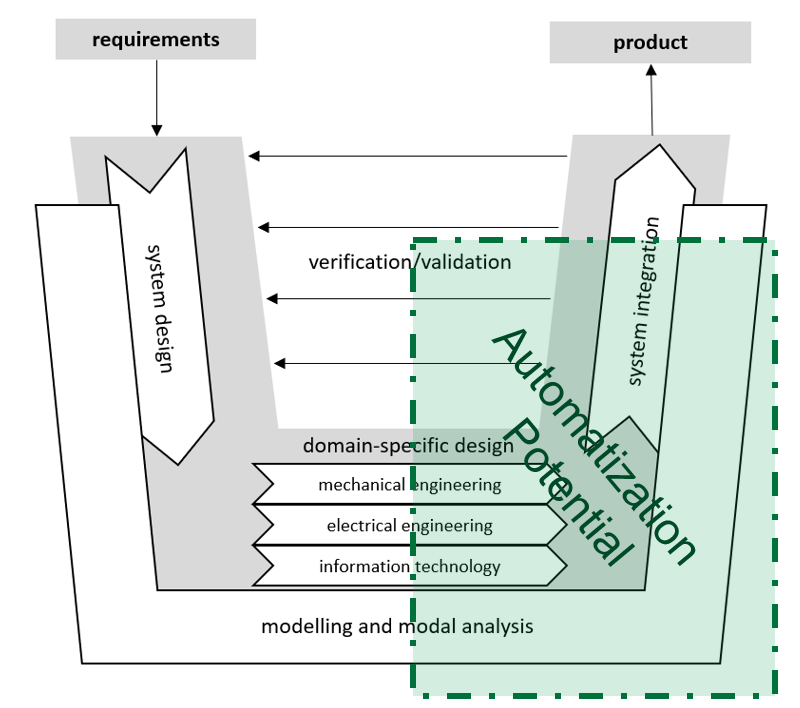
\includegraphics[scale=0.5]{pics/VDI_2206.PNG}
    \caption{\label{pic:VDI2206} "General approach for development and construction (VDI 2221)." \cite{Jansch2006THEDO}}
\end{figure}

ahnsdkjhauish
\section{Discussion}

asdas
\section{Conclusion}

Lightweight design requires highly optimized components.
These components therefore often need to go through a large amount of optimization cycles that are expensive and time consuming.
Therefor a proof of concept was introduced, which implements state of the art algorithm to increase to maximize the automation during the development process.
Further, the POC uses a scalable API system to enable information flow across development domains and 
In order to automate these steps, a software tool was introduced that can solve a given information based network of different processes.
Therefore, systems and solutions from disciplines such as graph theory and model representation in simulations were adapted to illustrate the development process.
In this work, a solving algorithm was introduced with which the connected sub-process can be processed, taking into account the interaction between the processes.
Further, the software was implemented to prove the predicted improvements in a high optimized, multi-domain environment.\\
In order to enable a broad use of the developed tool, the architecture was designed as modular as possible.
This meant that every simulation program, CAD-tool and digital process could be integrated into the design process.
Additionally, this approach also enables the software to easily be implemented in existing workflows, as existing models, files, etc. can be reused outside the developed software.
Further, the software uses a server-client network architecture to enable the specialists to collaborate on problems with with multiple domains and to outsource time-consuming operations to specialized servers.
Two examples demonstrate the capabilities for solving complex multi-domain problems and for finding optimal solutions.\\
The successful test shows a great work relief and time savings.
However, the developed tool has certain limitations and requires the ability to design products that some engineers are unfamiliar with.
For example, it is difficult, if not impossible, to implement manufacturing processes and experimental verification into the automatic design approach.
Additionally, engineers need to be able to express the value of a product, not necessary in relation to cost, as a mathematical formula so that the program can determine which solution is better.\\
Given the enormous potential of software driven solutions such as the tool developed, it is very likely that these kind of tools will become an essential part of every engineer's work routine.
However, improvements still made to be in terms of useability, performance, security, stability, and plugin support.\\
The authors would like to especially thank the University of Applied Sciences Leipzig, Germany
for the Funding as well as the DCIM- Dresden Center of Intelligent Materials, Germany
providing the A-frame specimens, as well as Jonas Richter, Andreas 
Hornig, and Xiaoang Si for helping with the simulation study (Institute 
of Lightweight Engineering and Polymer Technology, TU Dresden). We 
would also like to thank the Institute of Mechanical Process Engineering 
and  Mineral Processing  at  TU  Bergakademie  Freiberg,  Germany  for 
technical support and scientific discussions. We especially thank Tony 
Lyon, who assisted at the shredding experiments, and the research group 
on mechanical processing under Dr. Thomas Muetze. Gratitude is also 
expressed towards Dr. Hans-Georg Jaeckel and Dr. Christina Meskers for 
discussions and support in the early stages of this research, which helped 
to improve this work. 
\section*{List of Symbols}
\begin{table}[H]
    %\caption{\label{tb:los} A list of coordinates, which was used to generate the different degrees of deformation.}
    \centering
\begin{tabular}{c | c } 
    \toprule
    \textbf{symbol} & \textbf{meaning} \\ [0.5ex] 
    \midrule
    h & height\\
    J & Jacobian matrix\\
    m & Weibull module\\
    N & interpolation matrix\\
    NoE & number of elements\\
    NoN & number of nodes\\
    n & shape function\\
    $\sigma$ & stress\\
    V & Volume\\ 
    x, y & global coordinates\\
    $\xi$, $\eta$ & natural/local coordinates\\[1ex]
    \bottomrule
\end{tabular}
\end{table}

\section*{List of Indices}
\begin{table}[H]
    \centering
\begin{tabular}{c | c} 
    \toprule
\textbf{index} & \textbf{meaning} \\ [0.5ex] 
\midrule
$eff$ & effective\\
$f$ & rapture or failure\\
i & element number\\
j & node index in element\\
k & index of principle stress\\
$max$ & maximum\\ [1ex] 
\bottomrule
\end{tabular}
\end{table}

%\section*{acknowledgements}
%Acknowledgements should include contributions from anyone who does not meet the criteria for authorship (for example, to recognize contributions from people who provided technical help, collation of data, writing assistance, acquisition of funding, or a department chairperson who provided general support), as well as any funding or other support information.
%\printendnotes%???????????????????????????
% Submissions are not required to reflect the precise reference formatting of the journal (use of italics, bold etc.), however it is important that all key elements of each reference are included.
\bibliography{sources}
%\include{appendix}
\end{document}
